\section{pgaccess.c}
Trong hệ điều hành hay ở một số bộ thu gom rác phía người dùng, chương
trình cần biết trong khoảng thời gian vừa qua những trang nhớ nào đã bị
đọc hoặc ghi \cite{hcmus_os_lab3,mitpgtbl}. Trên kiến trúc RISC-V Sv39,
phần cứng có sẵn bit \code{PTE\_A} nằm ở vị trí bit thứ $6$ trong mỗi
PTE \cite{riscvspec}. Khi CPU truy cập vào một trang và gặp TLB miss,
phần cứng sẽ tự động bật bit \code{PTE\_A} từ $0$ lên $1$. Tuy nhiên,
phần cứng chỉ biết bật lên $1$ chứ không tự tắt về $0$, và tiến trình
user cũng không được phép đọc hay sửa trực tiếp bảng trang của kernel.
Vì vậy, ta cần thêm system call \code{pgaccess()} để kernel kiểm tra bit
\code{PTE\_A} giúp user, gom lại vào một bitmask rồi tắt \code{PTE\_A}
về $0$ cho lần kiểm tra sau.

\subsection{Triển khai}
Để bắt đầu, trong file \texttt{kernel/riscv.h}, ta định nghĩa cờ
\code{\#define PTE\_A (1L << 6)} có giá trị bằng $64$. Nhóm dùng
\code{1L} thay vì \code{1} để hằng số mang kiểu $64$ bit giống
\code{pte\_t}, giúp phép đảo bit \texttt{\textasciitilde{}PTE\_A} không
làm sai các bit cao khi xóa cờ. Tiếp đó, ta đăng ký system call mới
bằng cách thêm \code{SYS\_pgaccess = 25} vào \texttt{kernel/syscall.h},
khai báo \code{sys\_pgaccess()} rồi gắn vào bảng \code{syscalls[]} cùng
mảng \code{syscall\_names[]} trong \texttt{kernel/syscall.c}, đồng thời
khai báo \code{pgaccess(void *base, int len, void *mask);} trong
\texttt{user/user.h} và thêm \code{entry("pgaccess");} vào
\texttt{user/usys.pl}.

\paragraph*{Quét PTE và tắt cờ truy cập:} Khi user gọi
\code{pgaccess()}, hàm \code{sys\_pgaccess()} ở trong
\texttt{kernel/sysproc.c} dùng \code{argaddr(0, \&base)},
\code{argint(1, \&len)} và \code{argaddr(2, \&mask\_addr)} để lấy ba
tham số từ thanh ghi. Vì biến bitmask \code{curMask} dùng kiểu
\code{uint} dài $32$ bit, ta kiểm tra nếu \code{len < 0 || len > 32}
thì trả về $-1$ để tránh tràn bitmask hoặc lặp với số trang âm.

Tiếp theo, hàm khởi tạo \code{uint curMask = 0} và chạy vòng lặp
\code{i} từ $0$ đến \code{len - 1}. Ở mỗi bước, địa chỉ ảo đầu trang
thứ \code{i} được tính bằng \code{base + i * PGSIZE}. Nếu địa chỉ này
lớn hơn hoặc bằng \code{MAXVA}, hàm trả về $-1$ trước khi gọi
\code{walk()} vì đầu hàm \code{walk()} trong \texttt{kernel/vm.c} sẽ
gọi \code{panic("walk")} nếu nhận địa chỉ vượt quá \code{MAXVA}. Sau
đó, ta gọi \code{walk(p->pagetable, va, 0)} với tham số \code{alloc =
0} để chỉ tra tìm ô PTE đang có; nếu trang đó chưa được ánh xạ thì
\code{walk()} trả về $0$ chứ không tự ý gọi \code{kalloc()} tạo bảng
trang mới.

Khi có được con trỏ \code{pte}, hàm kiểm tra đồng thời \code{pte != 0},
\code{(*pte \& PTE\_V)} và \code{(*pte \& PTE\_A)}. Nếu cả ba đều đúng
thì trang này vừa được truy cập, ta bật bit thứ \code{i} trong
\code{curMask} bằng \code{curMask |= (1U << i)} (dùng \code{1U} để
dịch tới bit $31$ vẫn hợp lệ) rồi tắt ngay bit \code{PTE\_A} trong RAM
bằng \texttt{*pte \&= \textasciitilde{}PTE\_A} để lần gọi
\code{pgaccess()} sau không báo trùng trang cũ. Cuối cùng, do
\code{mask\_addr} là địa chỉ ảo bên user, kernel dùng \code{copyout()}
chép $4$ byte của \code{curMask} từ kernel ra \code{mask\_addr}; nếu
\code{copyout()} trả về số âm thì trả về $-1$, ngược lại trả về $0$.
Trình tự tương tác giữa tiến trình user, phần cứng MMU và
\code{sys\_pgaccess()} được mô tả trong Hình~\ref{fig:pgaccess_seq}.

\begin{figure}[H]
    \centering
    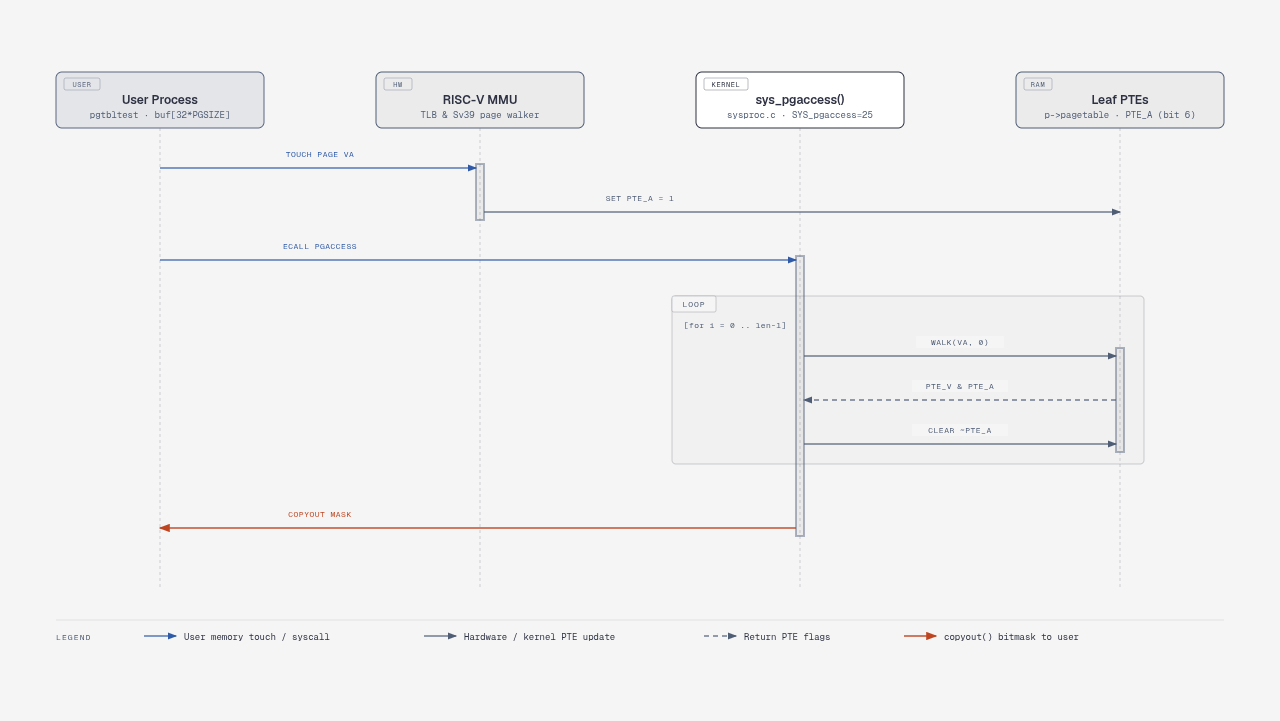
\includegraphics[width=0.96\textwidth]{images/pgaccess_seq.png}
    \caption{Luồng tương tác giữa user, MMU và \texttt{sys\_pgaccess()}
    khi đọc và xóa bit \texttt{PTE\_A}}
    \label{fig:pgaccess_seq}
\end{figure}

\subsection{Kiểm thử}
Để kiểm tra hoạt động của \code{pgaccess()} cùng với \code{ugetpid()}
trên QEMU, nhóm tạo file \texttt{user/pgtbltest.c} và khai báo vào
\code{UPROGS} của \texttt{Makefile}, bao gồm \code{ugetpid\_test()}
kiểm tra PID trên tiến trình cha và $64$ tiến trình con, cùng
\code{pgaccess\_test()} kiểm tra việc đọc, tắt \code{PTE\_A} và các
trường hợp biên (Bảng~\ref{tab:pgaccess_checks}).

\begin{table}[H]
    \centering
    \small
    \renewcommand{\arraystretch}{1.25}
    \begin{tabularx}{\textwidth}{p{0.38\textwidth} X}
        \toprule
        \textbf{Trường hợp kiểm tra} &
        \textbf{Mục đích kiểm tra} \\
        \midrule
        Gọi \code{pgaccess(buf, 32, \&abits)} ngay sau \code{malloc()} &
        Xóa sạch các bit \code{PTE\_A} còn sót lại từ lúc cấp phát bộ
        nhớ ban đầu trước khi đo. \\
        Ghi vào các trang $1, 2, 30$ rồi gọi \code{pgaccess()} &
        Kiểm tra giá trị \code{abits} nhận về khớp đúng với mặt nạ
        \code{(1U << 1) | (1U << 2) | (1U << 30)}. \\
        Gọi lại \code{pgaccess()} ngay sau đó mà không ghi thêm &
        Kiểm tra \code{abits == 0} để xác nhận kernel đã tắt bit
        \code{PTE\_A} về $0$ sau lần đọc trước. \\
        Ghi vào hai trang biên $0$ và $31$ rồi gọi lại &
        Kiểm tra \code{abits == ((1U << 0) | (1U << 31))}, bảo đảm
        đúng tới bit $31$ của kiểu \code{uint}. \\
        Truyền \code{len = -1}, \code{len = 33} hoặc con trỏ lỗi &
        Kiểm tra kernel chặn được tham số sai và lỗi \code{copyout()}
        bằng cách trả về giá trị âm mà không bị sập hệ thống. \\
        \bottomrule
    \end{tabularx}
    \caption{Các kịch bản kiểm thử trong \texttt{user/pgtbltest.c}}
    \label{tab:pgaccess_checks}
\end{table}

Khi chạy thực tế \texttt{pgtbltest} và \texttt{ugetpidtest} trên QEMU
(Hình~\ref{fig:pgtbltest_qemu}), tất cả các phần kiểm tra đều hoàn
thành và in ra thông báo đạt:
\begin{lstlisting}[style=terminalstyle]
$ pgtbltest
ugetpid_test starting
ugetpid_test: OK
pgaccess_test starting
pgaccess_test: OK
pgtbltest: all tests succeeded
$ ugetpidtest
getpid()  = 68
ugetpid() = 68
PID matched: 68
\end{lstlisting}

\begin{figure}[H]
    \centering
    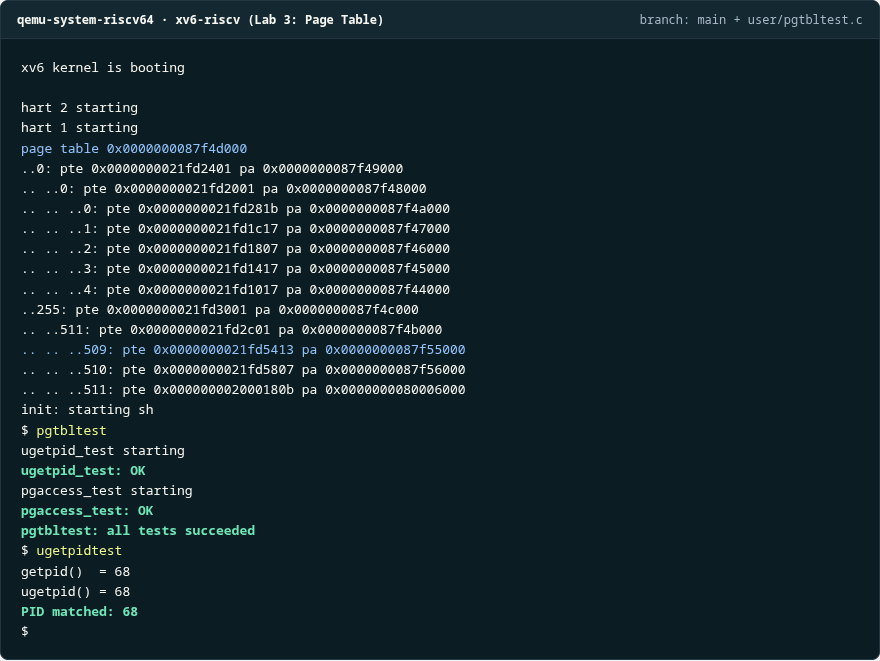
\includegraphics[width=0.84\textwidth]{images/pgtbltest-qemu.png}
    \caption{Kết quả chạy kiểm thử \texttt{pgtbltest} và
    \texttt{ugetpidtest} trên QEMU sau khi ghép đủ cả ba phần}
    \label{fig:pgtbltest_qemu}
\end{figure}
